\chapter{Исследовательская часть}

В данном разделе будут приведены технические характеристики устройства, на котором проводился анализ алгоритмов, а также результаты работы программного обеспечения.

\section{Технические характеристики}

Технические характеристики устройства, на котором выполнялось исследование, следующие:

\begin{itemize}[label=---]
	\item Операционная система: Microsoft Windows 10 Pro;
	\item Оперативная память: 32 ГБ;
	\item Процессор: Intel(R) Core(TM) i9-9980HK CPU @ 2.40GHz, 2401 Mhz;
	\item Количество ядер: 8 физических и 16 логических.
\end{itemize}

\section{Результаты работы ПО}

На рисунках \ref{img:4-1} -- \ref{img:4-3} представлены изображения, полученные с помощью разработанного ПО.

\begin{table}[H]
	\centering
	\begin{tabular}{p{1\linewidth}}
		\centering
		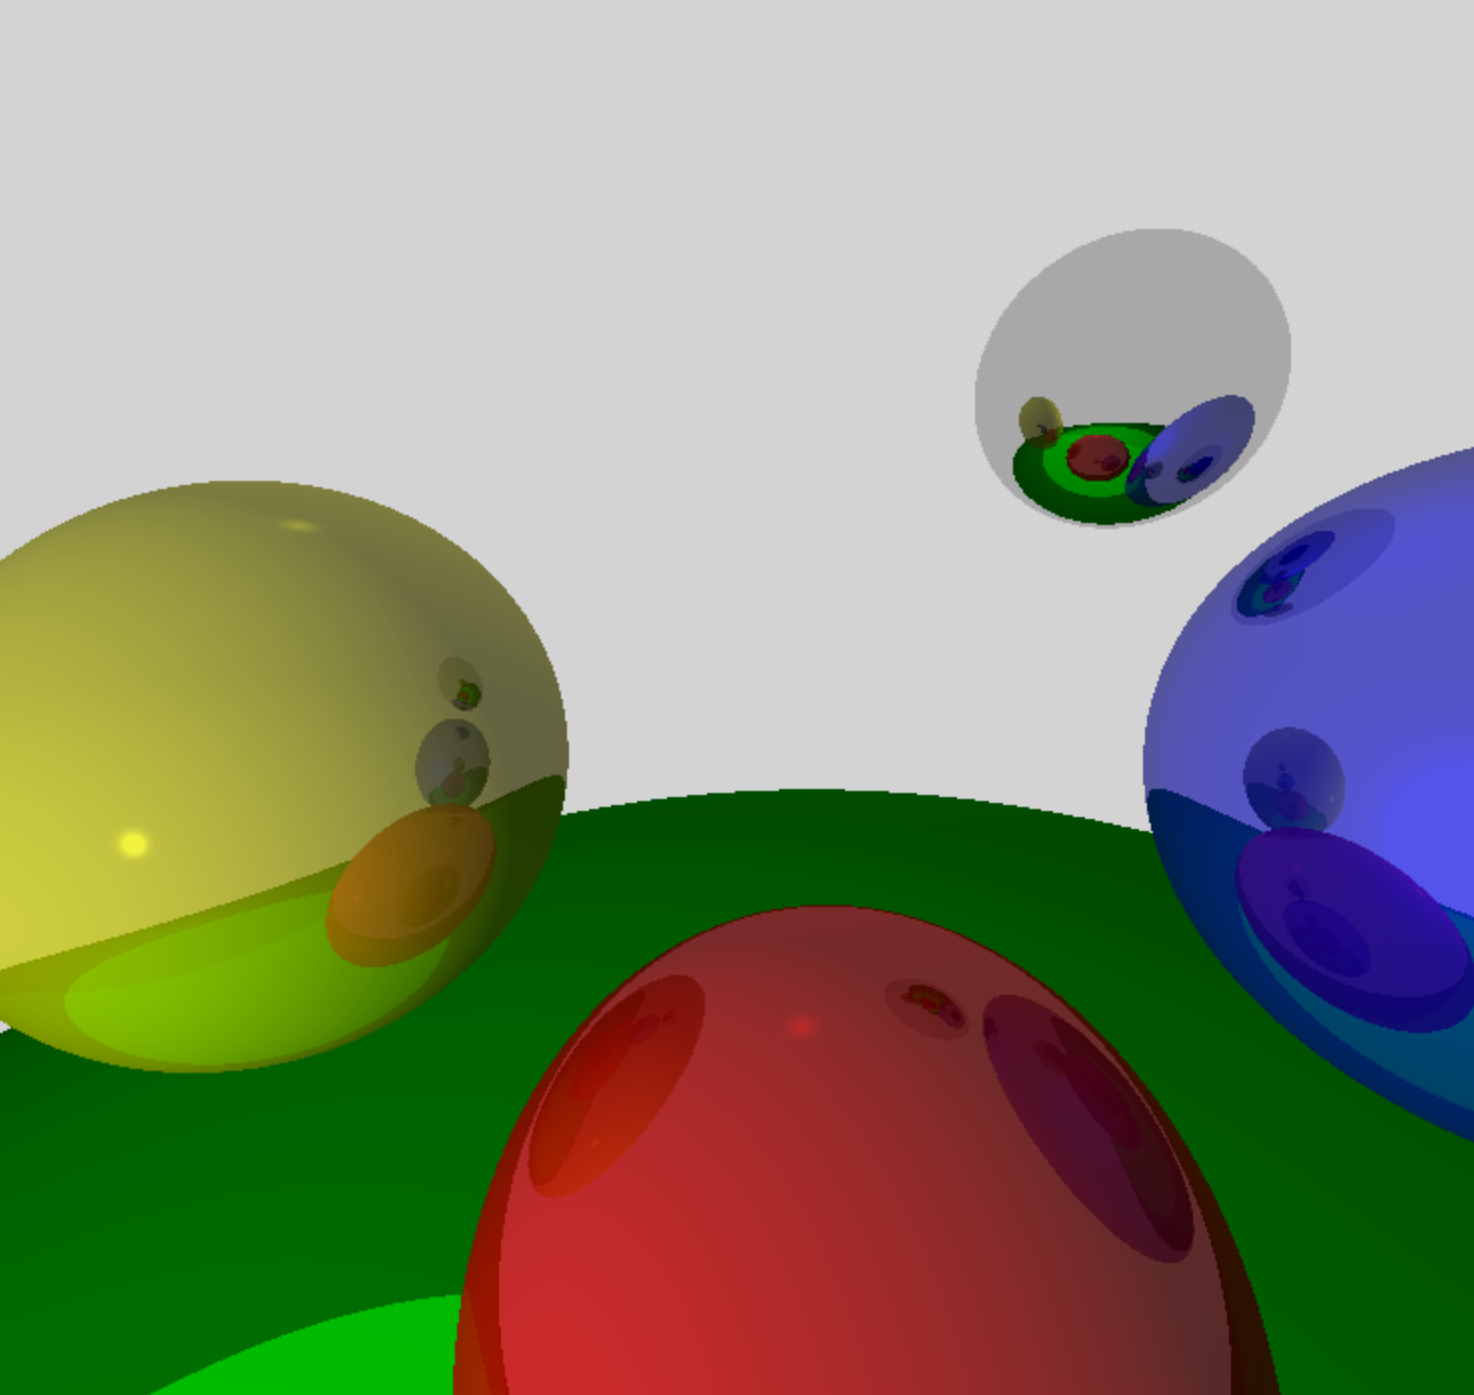
\includegraphics[width=0.7\linewidth]{include/4-1.png}
		\captionof{figure}{Отражение сфер друг от друга.}
		\label{img:4-1}
	\end{tabular}
\end{table}

\begin{table}[H]
	\centering
	\begin{tabular}{p{1\linewidth}}
		\centering
		
\includegraphics[width=0.6\linewidth]{include/4-2.png}
		\captionof{figure}{Отображение света.}
		\label{img:4-2}
	\end{tabular}
\end{table}

\begin{table}[H]
	\centering
	\begin{tabular}{p{1\linewidth}}
		\centering
		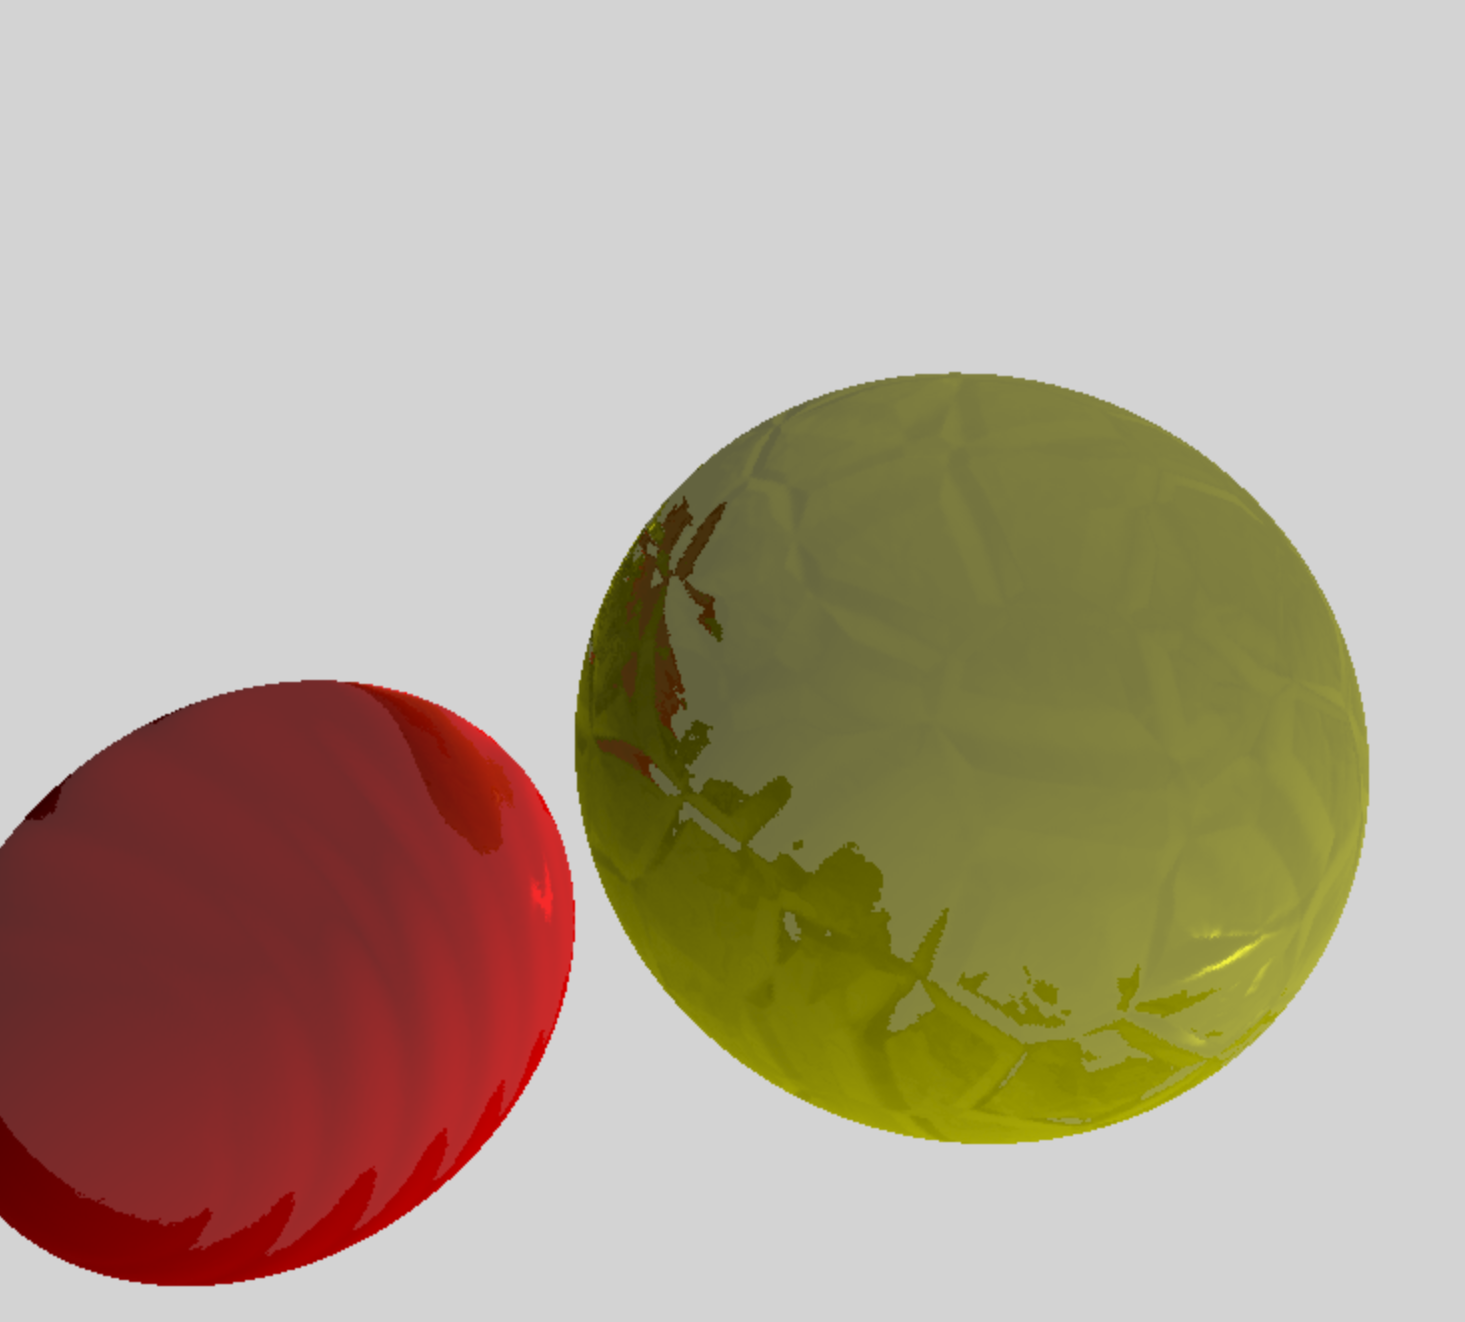
\includegraphics[width=0.7\linewidth]{include/4-3.png}
		\captionof{figure}{Простая композиция шаров с текстурами.}
		\label{img:4-3}
	\end{tabular}
\end{table}

\section{Анализ производительности}

Производительность будет оцениваться мерой количества кадров в секунду (FPS). Она будет меняться в зависимости от размера ткани. Количество кадров в секунду было замерено с помощью модуля \textit{Stats}. Результаты приведены в таблице \ref{tbl:profilingalgs1}. 

\begin{table}[H]
	\begin{center}
		\caption{\label{tbl:profilingalgs1} Производительность ПО при разном размере тканевой сетки.}
		\begin{tabular}{|c|c|}
			\hline
			\specialcell{Линейный размер ткани, частиц} & \specialcell{FPS}
			\\ 
			
			\hline
			100 & \num{60} \\ \hline
			500 & \num{60} \\ \hline
			1000 & \num{60} \\ \hline
			1500 & \num{60} \\ \hline
			2000 & \num{54} \\ \hline
			2500 & \num{49} \\ \hline
			5000 & \num{27} \\ \hline
		\end{tabular}
	\end{center}
\end{table}

Исходя из результатов, можно заметить понижение количества кадров в секунду при большом размере тканевой сетки. Это происходит в силу большой вычислительной нагрузки, так как требуется расчет траектории для каждой частицы ткани.

\section*{Вывод}
\addcontentsline{toc}{section}{Вывод}
В данном разделе приведен анализ производительности, а также результат работы программного обеспечения. В ходе анализа было установлено, что количество кадров в секунду уменьшается с увеличением размера ткани.